\documentclass[12pt, a4paper]{report}
\usepackage{graphicx, array, amsthm, amssymb, amsmath, float, xcolor, thmtools, thmbox, titling}
\usepackage[english]{babel}


\title{Design Document}
\author{Christian Rossi \\ Kirolos Sharoubim}
\date{Academic Year 2023-2024}

\begin{document}

\begin{titlingpage} 
    \begin{center}
        
\includegraphics[height=5cm]{images/polimi.png}\\
        \vspace{4cm}
        \begin{huge} 
            \textbf{\thetitle} \\
        \end{huge}
        \vspace{0.3cm}
        \begin{Large}
            \textit{Software Engineering 2 \\ CodeKataBattle} \\
        \end{Large}
    \end{center}
    \vspace{6.9cm}
        \begin{center}      
            \textbf{Authors}    

            Christian Rossi - 10736464   

            Kirolos Sharoubim - 10719510
    \end{center}
\end{titlingpage}

\newpage

\tableofcontents

\newpage

\chapter{Introduction}
    \section{Purpose}
    This document aims to provide a comprehensive insight into the CodeKataBattle system outlined in the RASD.
    It delves into the system's architecture, elucidating on its components,
    their interactions, processes, and algorithms designed to meet RASD requirements. 
    Furthermore, it offers explicit instructions pertaining to the implementation, integration, and testing plan. 
    Geared towards developers, testers, and project managers, this document serves as a valuable reference for the system's implementation phase.

    \section{Scope}
    CodeKataBattle serves as a platform utilized by educators to engage students in coding Katas - challenges designed to be addressed using a programming language specified by the challenge organizers. 
    Educators possess the capability to establish a code Kata within a particular tournament, defining essential parameters such as the problem statement (inclusive of test cases), 
    the minimum and maximum number of students allowed per group, and the deadlines for both code Kata registration and solution submission.
    Following the tournament creation, students are empowered to create groups and commence their collaborative efforts on the solution, following a test-first approach. 
    As the ultimate deadline approaches, the system autonomously computes the final rankings, ultimately revealing the victorious participants.
    For a more comprehensive overview of the features accessible to end users, please consult the RASD. 
    The architecture of the S2B is structured into three physically separated layers, each installed on distinct tiers. These layers are:
    \begin{enumerate}
        \item \textit{Presentation Layer}: Responsible for overseeing the presentation logic and handling all interactions with end users.
        \item \textit{Business Logic Layer}: Manages the application functions provided by the S2B, ensuring seamless operation and functionality.
        \item \textit{Data Layer}: Handles secure storage and facilitates access to data, ensuring the integrity and reliability of information.
    \end{enumerate}

    \section{Definitions, acronyms and abbreviations}
    \subsection{Definitions}
    \textbf{Code Kata}: adaptation of the concept of karate katas, where you repetitively refine a form, to the realm of software development, 
        fostering iterative practice and improvement. 
    \\
    \textbf{Test-first approach}:  software development process relies on the transformation of software requirements into test cases before 
        the software is completely developed, and it involves monitoring the entire software development by iteratively testing the software 
        against all these test cases.
    \subsection{Acronyms}
    \textbf{CKB}: CodeKataBattle 
    \\
    \textbf{CK}: Code Kata
    

    \section{Revision history}
    \textbf{Version 1.0} - Release - date 22/12/2023


    \section{Reference documents}
    \textbf{Document 1} - Presentation about RASD structure
    \\
    \textbf{Website 1} - http://codekata.com
    \\
    \textbf{Website 2} - https://en.wikipedia.org


    \section{Document structure}
    This document comprises seven sections:

    \begin{enumerate}
        \item \textit{Introduction}: This section furnishes an overview of the Design Document (DD), encompassing the project's scope, key term definitions, references to pertinent documents, and a brief outline of the design. 
        \item \textit{User Interface Design}: Outlining the design of the user interface (UI) along with user experience (UX) flowcharts, this section provides a detailed perspective on how users will interact with the system. 
        \item \textit{Architectural Design}: Describing the high-level components and interactions within the system, this section includes a component view, deployment view, runtime view, and insights into selected architectural styles and patterns.
        \item \textit{Requirements Traceability}: Establishing a clear connection between the requirements specified in the Requirements and Specification Document (RASD) and the components outlined in the DD, this section ensures traceability throughout the design process.
        \item \textit{Implementation, Integration, and Test Plan}: This section details the plan for implementing, integrating, and testing the system. It includes the sequence in which subsystems and components will be implemented, providing a roadmap for the development process.
        \item \textit{Effort Spent}: Offering insights into the effort invested in the design process, this section provides information on the resources and time dedicated to the various aspects of the design.                 
        \item \textit{References}: This section encompasses a list of references cited within the Design Document, providing a foundation for further exploration and understanding.
    \end{enumerate}   
    
\newpage 

\chapter{Architectural design}
The purpose of this section is to systematically present and assess the architecture of the S2B system in a top-down approach. 
    We first introduce the comprehensive architecture and then provide a diagram illustrating the system's components, with a specific emphasis on the Educators and students subcomponents. 
    Subsequently, we employ an Entity-Relationship (ER) diagram to articulate the system's logical data and present the system's deployment view, encompassing layers and tiers. 
    We also use sequence diagrams to illustrate crucial runtime perspectives, while class diagrams are employed to scrutinize the interfaces of the components. 
    Ultimately, we engage in a discussion on the architectural design choices and the rationale behind them.
    \section{Overview}
    The diagram below provides a high-level depiction of the components that form the System. 
    In this document, we will use the term "Frontend" to encompass both the presentation layer and the Client 
    (e.g., the Browser), while the term "Backend" will encompass both the Application Layer and the Data Layer.
    \begin{figure}[H]
        \centering
        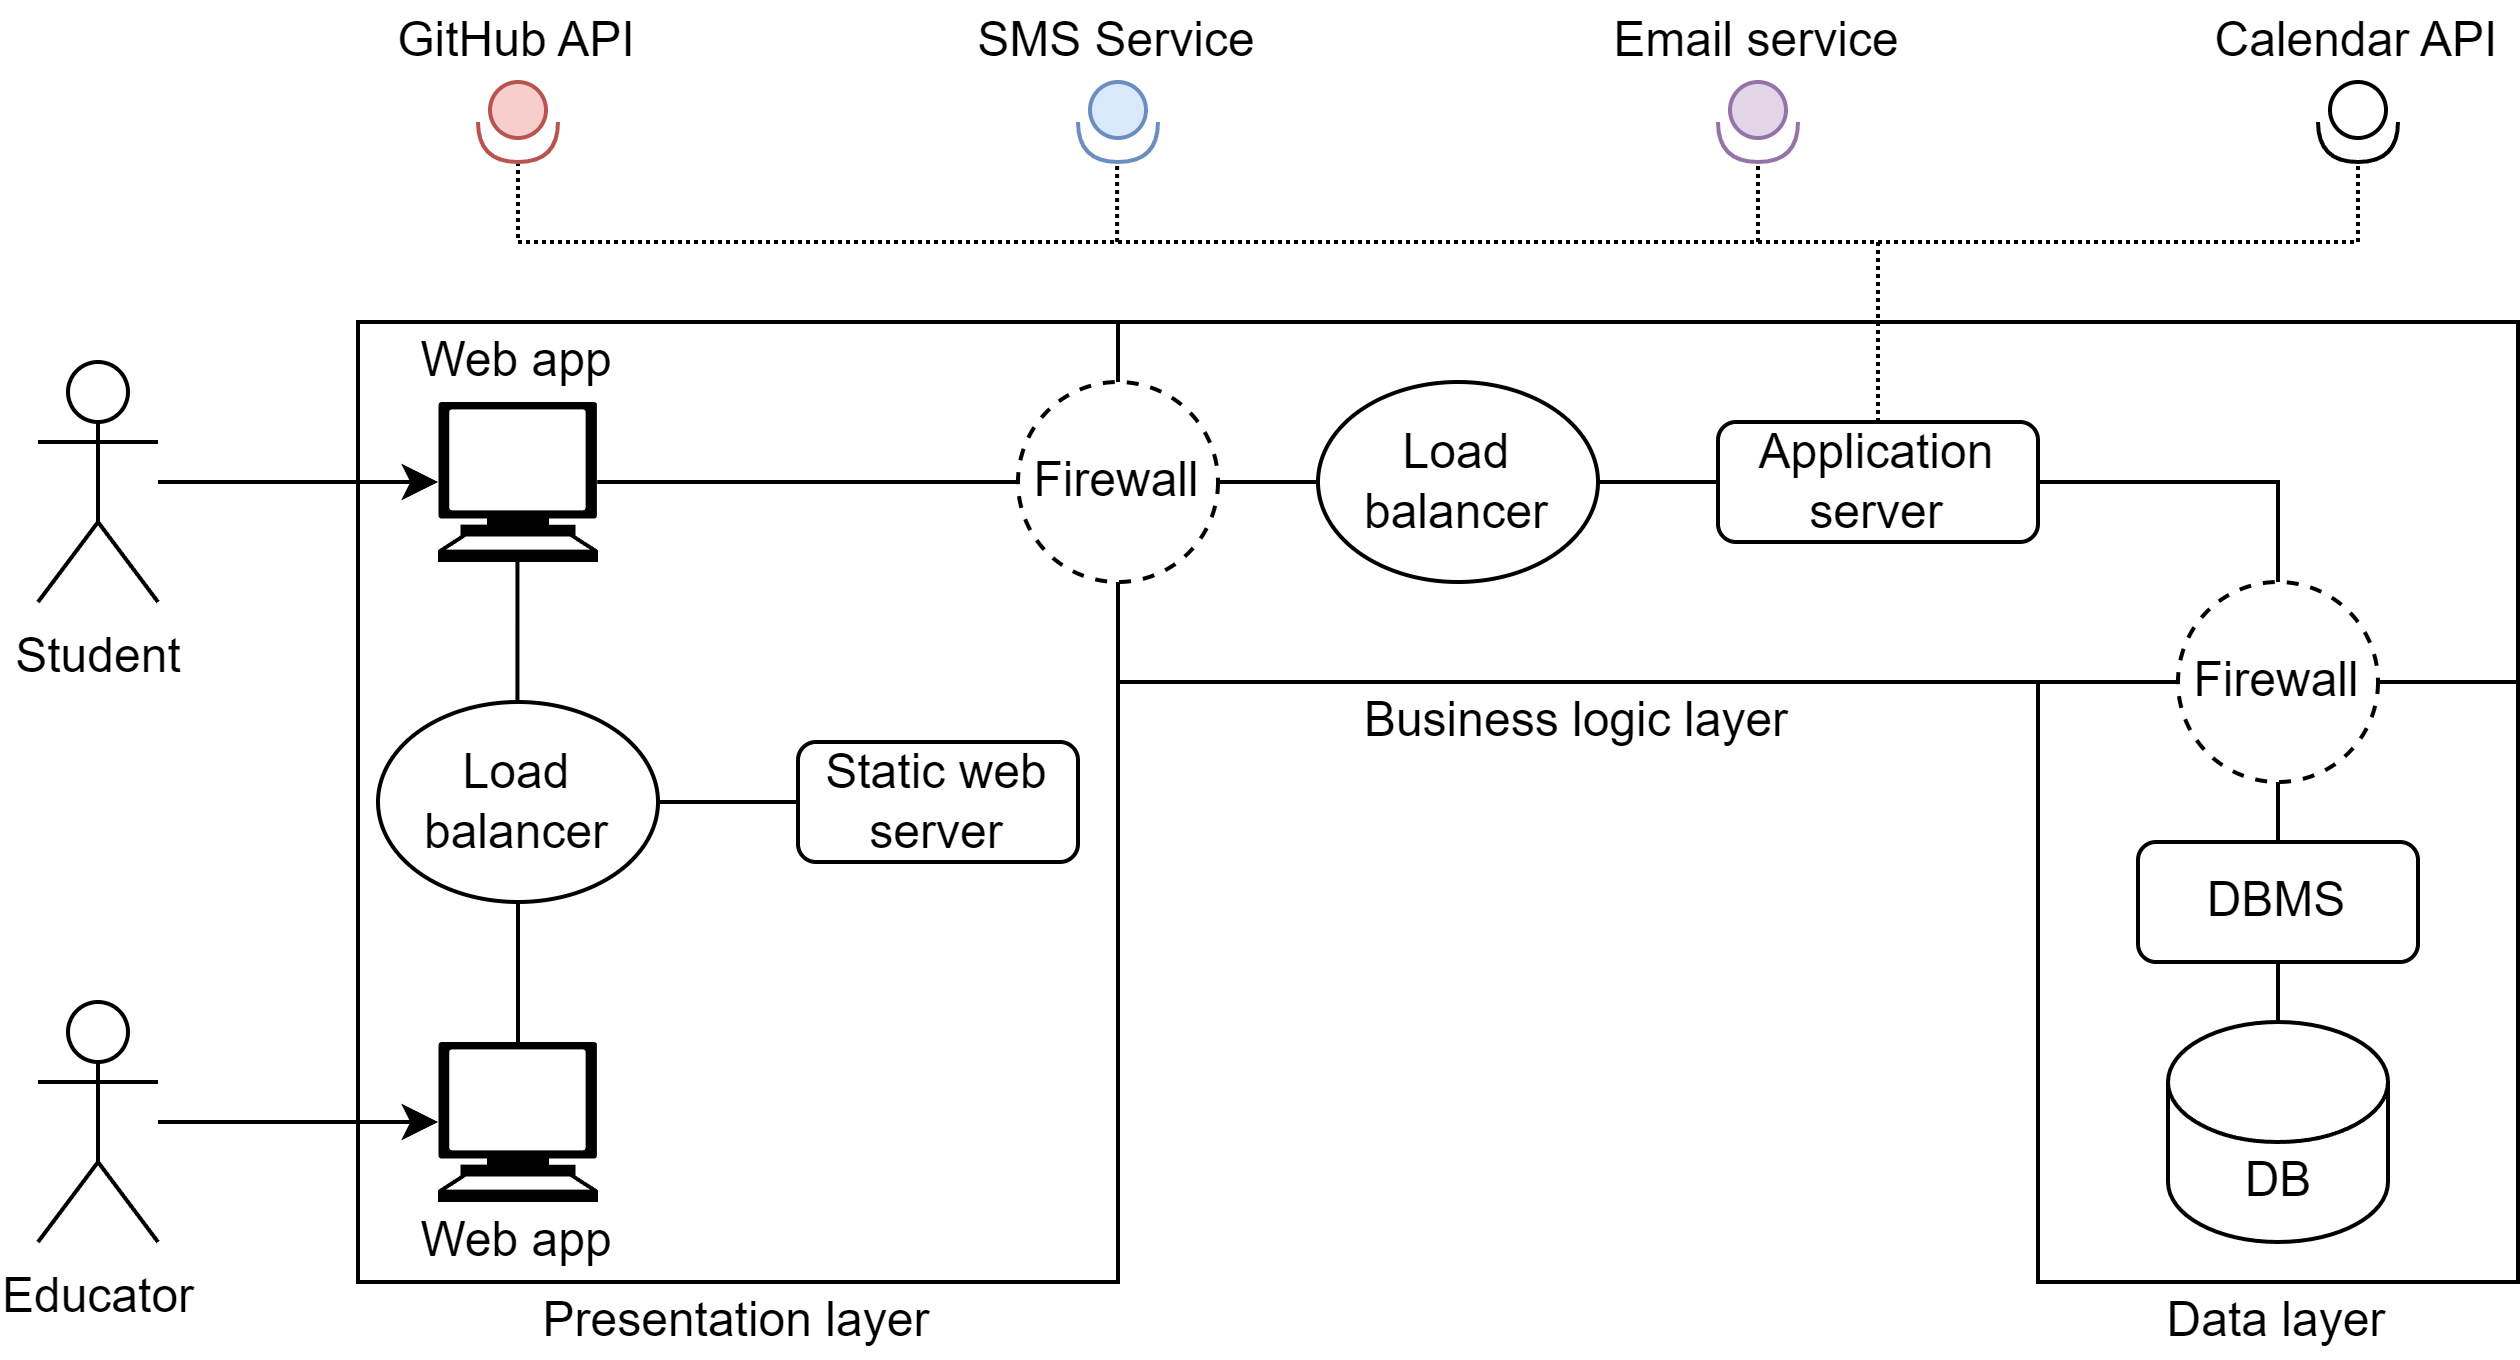
\includegraphics[width=1.0\linewidth]{images/high_level_architecture.png}
    \end{figure}
    \section{Component view}
    The service will be accessed through a web interface, utilizing a single page application (SPA) that proves advantageous for this application type, 
    enabling extensive interaction without frequent page reloads, thereby ensuring a faster and smoother user experience. 
    The system's architecture is structured three into distinct layers, with application servers interacting 
    with a database management system and utilizing APIs for data retrieval and storage. Adhering to REST standards, 
    the application servers are designed to be stateless, and the system incorporates firewalls to bolster security.
    \section{Deployment view}
    \section{Runtime view}
    \section{Component interfaces}
    \section{Selected architectural styles and patterns}
    \section{Other design decisions}

\newpage 

\chapter{User interface design}
    The user interface is the visual representation of how the application appears to the end user.
    It should be intuitive and straightforward, ensuring easy access to all features.
    Mockups were introduced in the RASD document, and now flowcharts for both students and educators will be presented.
    Flowcharts offer a concise and clear overview of the interactions and steps involved in utilizing the web app.
    \section{Flowchart for students UI}
    \begin{figure}[H]
        \centering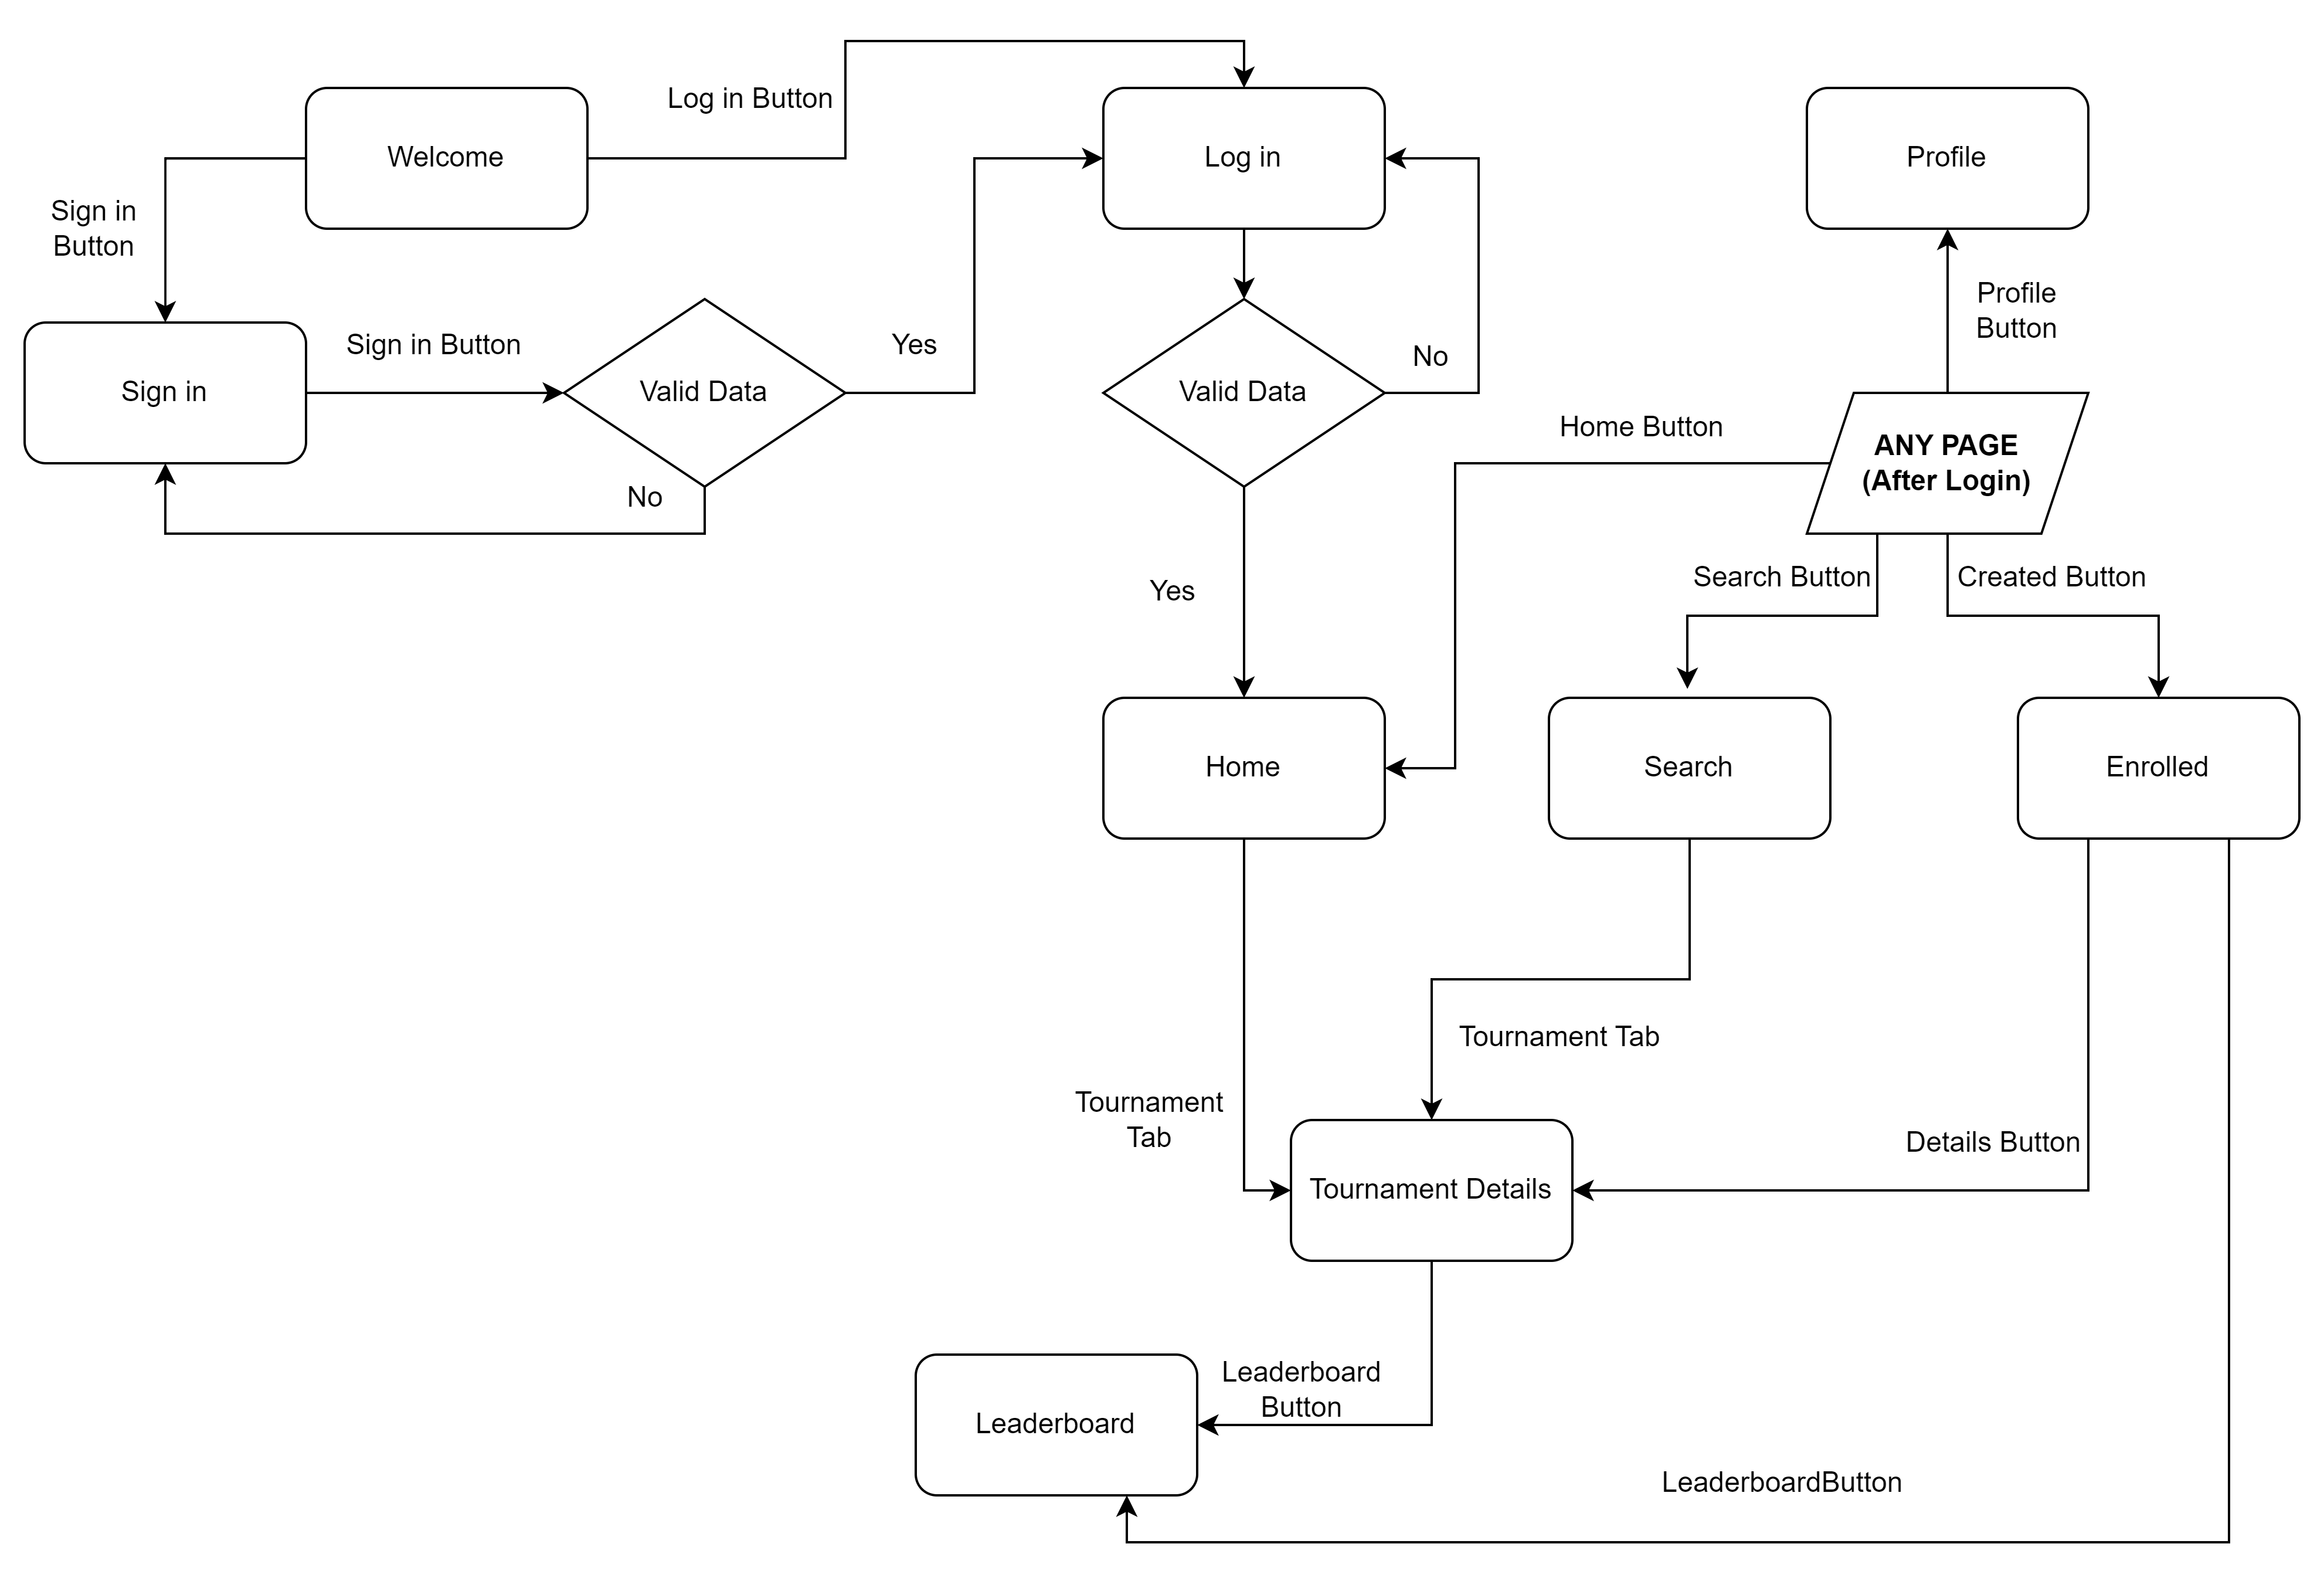
\includegraphics[width=0.9\linewidth]{images/students_UI.png}
    \end{figure}
    \section{Flowchart for educators UI}
    \begin{figure}[H]
        \centering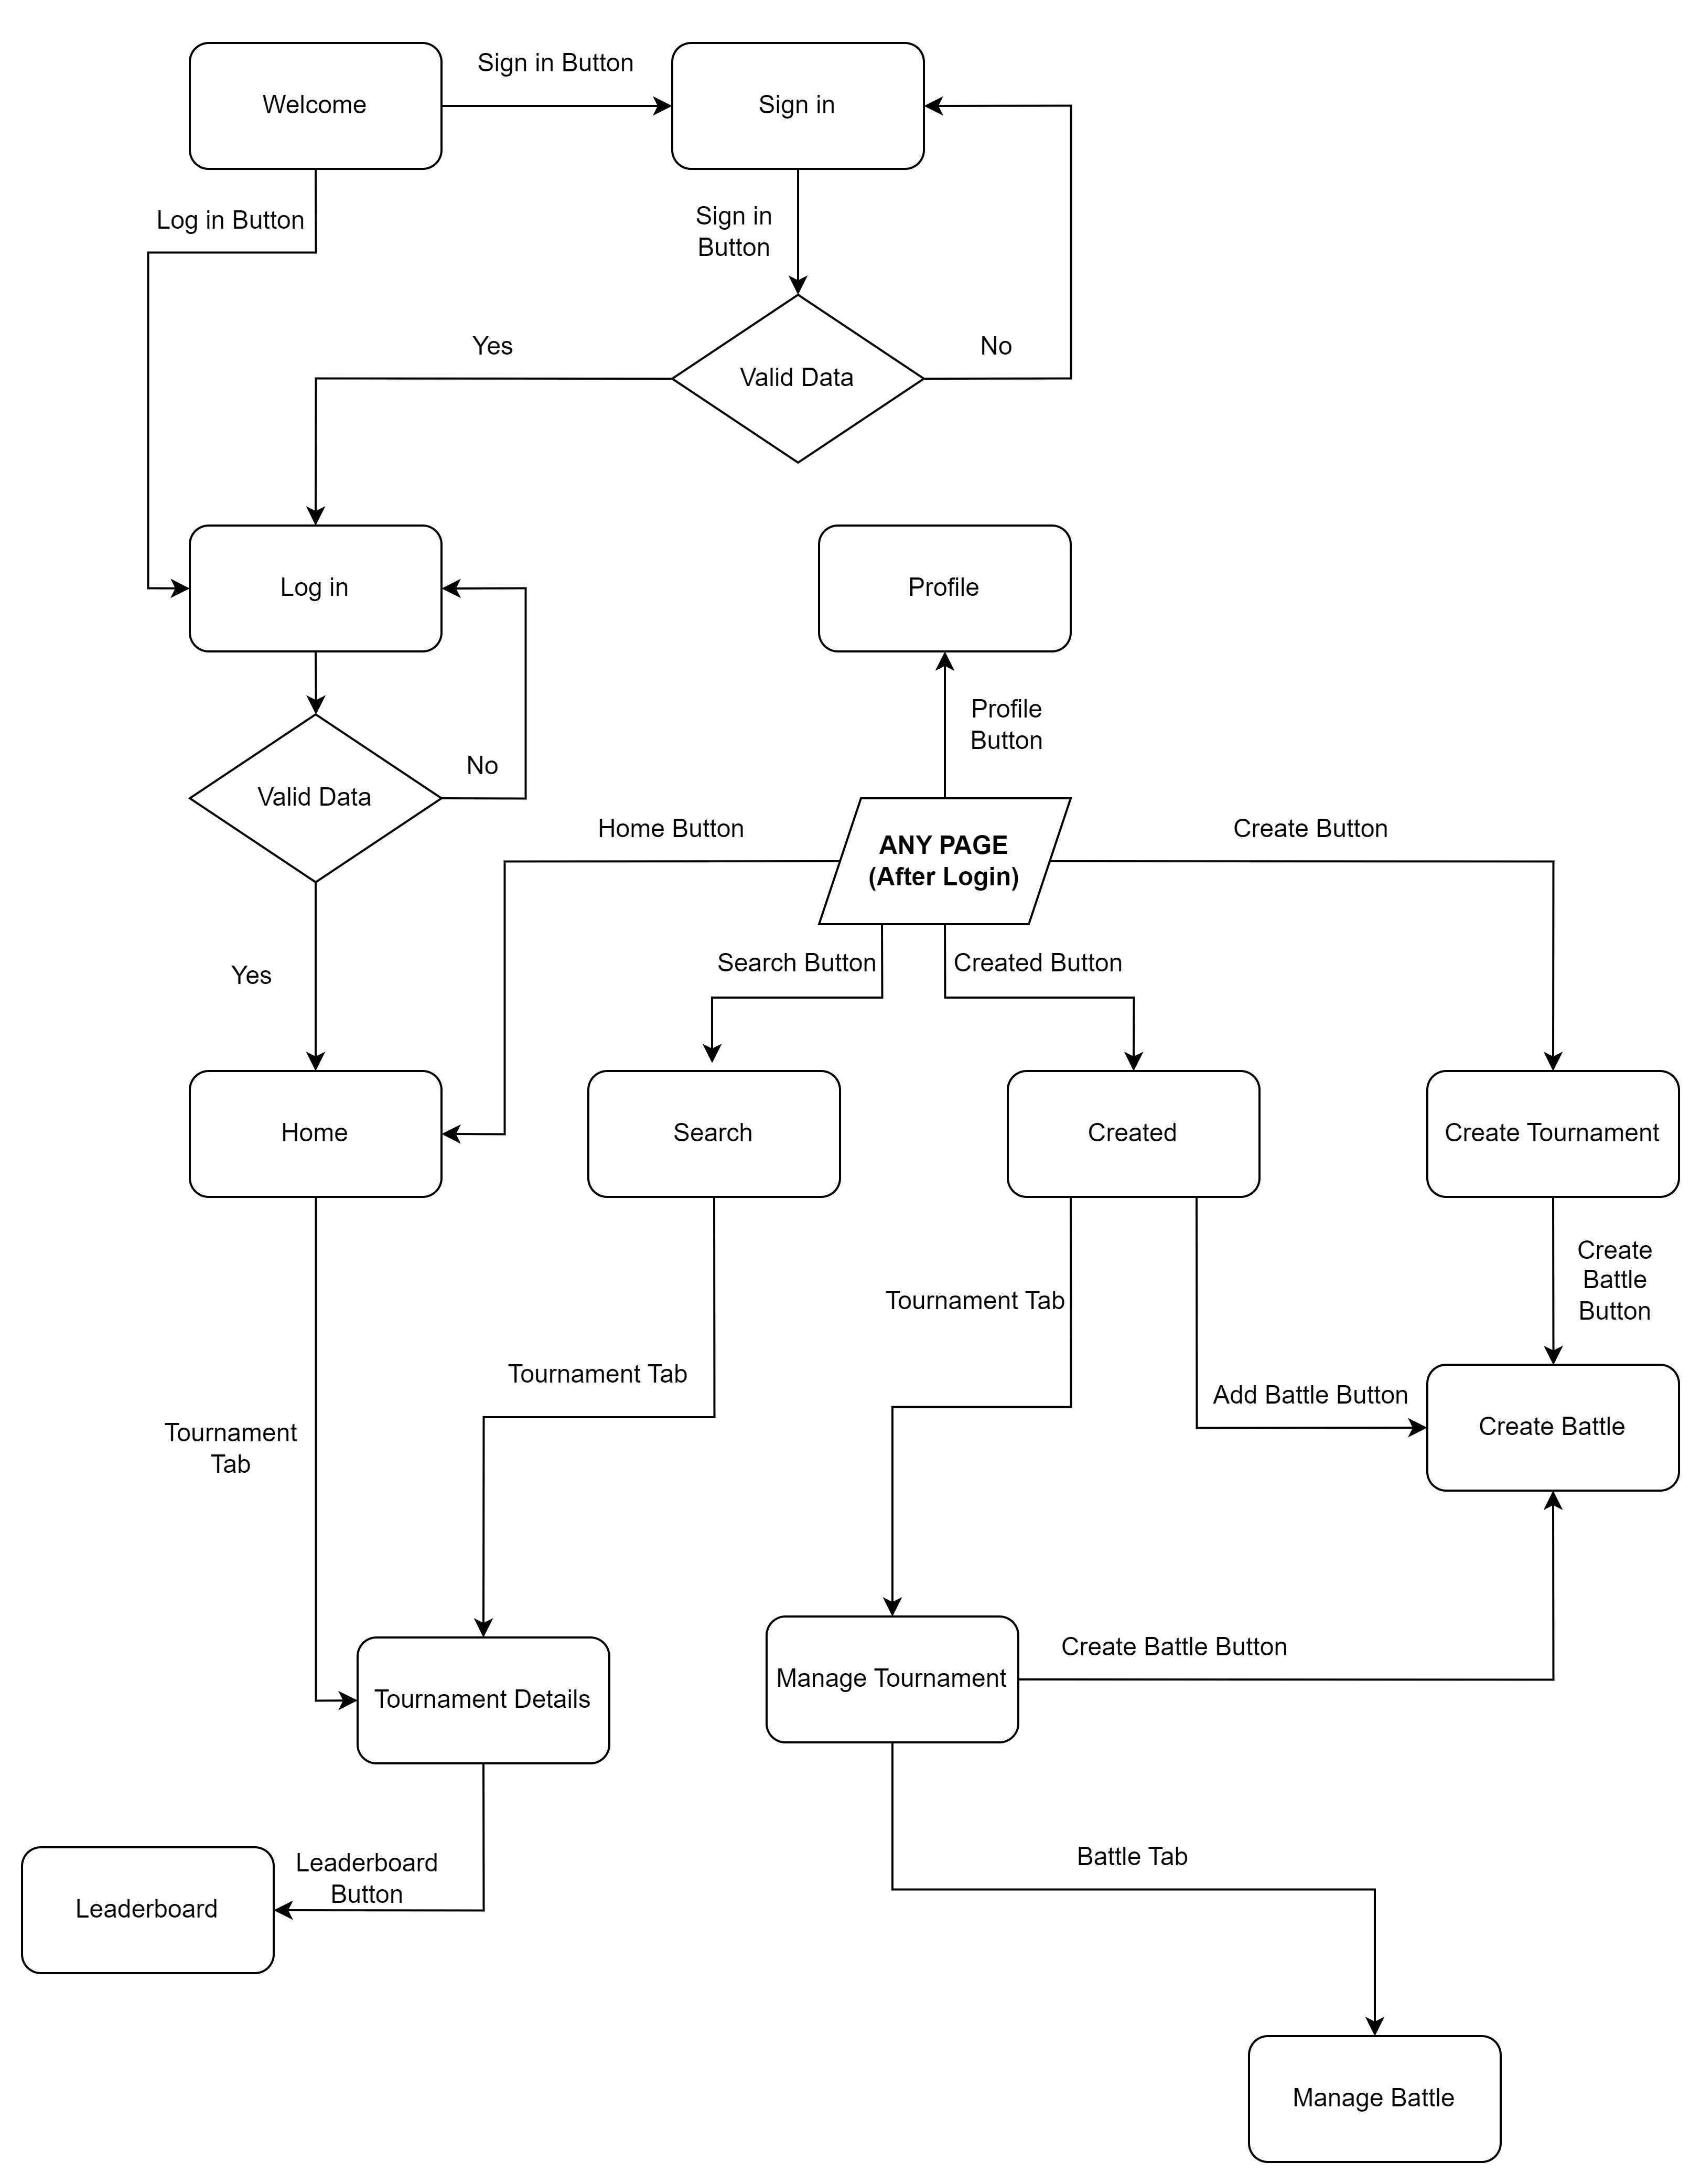
\includegraphics[width=0.9\linewidth]{images/educators_UI.png}
    \end{figure}

    \newpage 

\chapter{Requirements traceability}

\newpage 

\chapter{Implementation, integration and test plan}

\newpage 

\chapter{Effort spent}

\newpage 

\chapter{References}

\end{document}